\documentclass[conference]{IEEEtran}
\IEEEoverridecommandlockouts
% The preceding line is only needed to identify funding in the first footnote. If that is unneeded, please comment it out.
\usepackage{cite}
\usepackage{amsmath,amssymb,amsfonts}
\usepackage{algorithmic}
\usepackage{graphicx}
\usepackage{textcomp}
\usepackage{xcolor}
\usepackage{bm}
\usepackage{subcaption}
\usepackage{listings}
\usepackage{framed}
\usepackage{hyperref} 
\usepackage{lettrine}
\def\BibTeX{{\rm B\kern-.05em{\sc i\kern-.025em b}\kern-.08em
    T\kern-.1667em\lower.7ex\hbox{E}\kern-.125emX}}

\begin{document}

\title{\textbf{In-Memory Sorting and Searching with Akers Array}\\
% {\footnotesize \textsuperscript{*}Note: Sub-titles are not captured in Xplore and
% should not be used}
% \thanks{Identify applicable funding agency here. If none, delete this.}
}

\author{
 \IEEEauthorblockN{Kasturi Dikpati}
 \IEEEauthorblockA{\textit{Information Technology} \\
 \textit{University Institute of Technology}\\
 Burdhawan, India \\
 kasturi.dikpati@gmail.com}
\and
\IEEEauthorblockN{Barnik Roy}
\IEEEauthorblockA{\textit{Computer Science and Technology} \\
\textit{IIEST, Shibpur} \\
Howrah, India \\
thunderburning987@gmail.com}
\and
\IEEEauthorblockN{Pantho Propan Debnath}
\IEEEauthorblockA{\textit{Computer Science and Technology} \\
\textit{IIEST, Shibpur} \\
Howrah, India \\
panthonath12179@gmail.com}
\and
\IEEEauthorblockN{Biplab K. Sikdar}
\IEEEauthorblockA{\textit{Computer Science and Technology} \\
\textit{IIEST, Shibpur} \\
Howrah, India \\
biplab@cs.iiests.ac.in} 
}

\maketitle

\begin{abstract}
In the realm of efficient data management, sorting and searching algorithms play a crucial role in optimizing performance. This work presents a comprehensive study of in-memory sorting and searching using the Akers logic array, a two-dimensional structure capable of parallel computation through configurable logic cells. We extend the capabilities of the Akers array beyond binary sorting to support generalized (non-binary) sorting, and further implement both linear and binary search operations within the same framework. A conceptual memory architecture is also proposed, partitioning the Akers array into Stasis and Flux regions to differentiate between storage and computation zones. Our approach reveals significant improvements in execution time and resource efficiency when implemented in hardware, offering a scalable and reconfigurable solution for high-performance, data-centric applications. These insights pave the way for future innovations in in-memory computing and hardware-level algorithm optimization.


\end{abstract}

\begin{IEEEkeywords}
Akers array, in-memory-computation, sorting, cellular logic, combinatorial logic, parallel processing.
\end{IEEEkeywords}

\section{Introduction}

In recent years, computing architectures have undergone significant transformation, moving away from the conventional von Neumann model toward innovative designs that integrate processing and memory functionalities and effectively realized in-memory computation that conventionally done by the CPU. Tthe Akers logic array, introduced by Sheldon Akers in 1972 \cite{5009040}, which facilitates the execution of Boolean functions through a network of primitive logic cells. Each cell within this grid features three inputs and two outputs, facilitating the dynamic introduction of external input variables.

 This work presents a two-dimensional array of identical logic cells designed to meet these evolving requirements while retaining the beneficial characteristics of Akers arrays. Through careful configuration of input variables across the array,a systematic method for synthesizing combinatorial switching functions is developed that leads to realization of in-memory sorting.

To showcase the practicality of the Akers logic array in data-intensive operations, the following sections delve into its core components and demonstrate its adaptability for in-memory computation. The paper begins by laying out the architecture of the Akers array, describing the structure and behavior of its logic cells, and how these cells interconnect to enable parallel execution of Boolean functions. With this foundation, we explore its application in sorting binary inputs using a triangular configuration and control logic, establishing the array’s baseline utility in basic in-memory operations.

Building upon binary sorting, the paper then transitions to more advanced use cases—namely, generalized sorting with non-binary symbols and implementing comparative operations using binary-coded data. These sections reveal how the Akers array supports the median function for multi-valued logic and facilitates fundamental sorting steps like min-max extraction. The analysis continues with a detailed treatment of search operations—both linear and binary—realized within the same logic framework, culminating in the conceptualization of a hybrid memory model with partitioned zones for storage (Stasis) and computation (Flux). Together, these sections underscore the versatility of Akers arrays in redefining memory and computation boundaries in modern hardware design.
\medskip

\section{Akers Array}

Akers array has been introduced by S. B. Akers in 1972. Such an Akers array is composed of identical logic cells interconnected in a rectangular grid, as shown in Figure \ref{fig:Akers-array}. Each cell has three inputs and two outputs. Two of the inputs are fixed connections --- immediately from up ($X$) and left ($Y$). The two outputs ($f$) are permanently connected to the two cells --- immediately to the right and down. The third input to the cell is an external input on which an arbitrary input variable ($Z$) may be introduced. This input is under the designer's control. By defining logical operation of the array cells in proper ways, several logic functions can be realized. However, it is to be expected that certain input combinations to the cells never occur.

\begin{figure}[h]
\centering
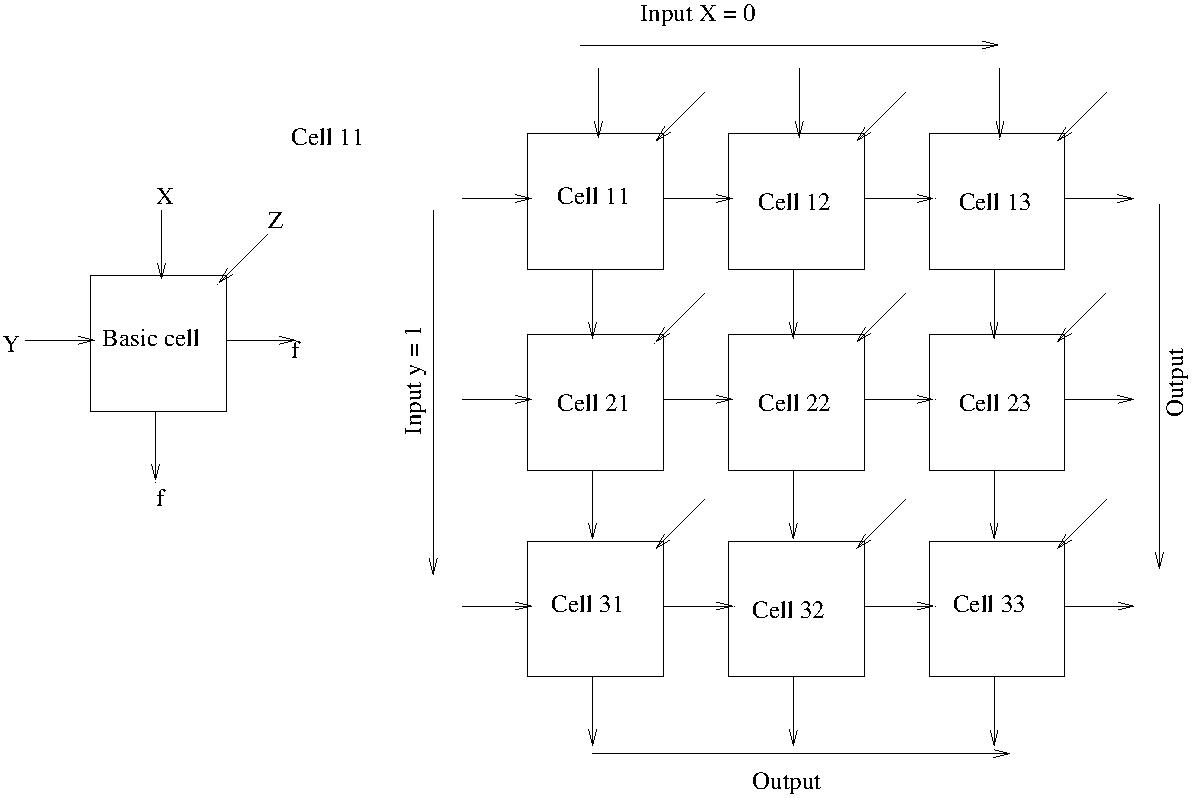
\includegraphics[width=0.5\textwidth]{akersarray.pdf}
\caption[Akers array]{\centering Akers array
\label{fig:Akers-array}}
\end{figure}

% A primitive Akers array cell can implement 1 of the 4 possible 3-input ($x$, $y$, $z$) and 1-output ($f$) logic functions, namely:
A binary Akers array cell implements only one out of the following four possible Boolean functions, 
\\$f(x, y, z): \{0,1\}^3 \to \{0, 1\}$, as defined in\cite{5009040}:
\begin{align*}
f &= y(x+z) \\
f &= z'x+zy \\
f &= xy+yz+zx \\
f &= x+yz
\end{align*}

\medskip

%%% UNCOMMENT AND USE LATER IF NEEDED

% \subsection{Software realization}
% \medskip

% As shown in the code snippet below, Python functions can effectively simulate the golden models for the basic operations of an Akers array cell at a high level.
% % Small test cases are written to automatically verify the functionality of each cell.
% \\\\
% \scalebox{0.9}{
%     \fbox{
%         \lstinputlisting[language=Python]{cell.py}
%     }
% }

% % \bigskip

% %\subsection{Low level (Using Verilog)}
% \medskip
% An example of a Verilog module designed to replicate an Akers array primitive cell is shown below:
% \\\\
% \scalebox{0.99}{
% \fbox{
%     \lstinputlisting[language=Verilog]{f1.v}
    
% }} 

% \bigskip

% Performing structural modeling on these primitive cells, an Akers array can be simulated. Fig. \ref{fig:large_diagram} illustrates an RTL design for such a simulated array.

\medskip

\section{binary sorting with akers array}
\medskip
Binary-sorting (bit sorting) with Akers array has been introduced in \cite{f1ed133a92fb4968b15110edea392daa}. A binary bit sequence of $n$ elements is --- $[ x_1, \ldots, x_n ]$. A triangular configuration above the minor diagonal of a square matrix of order $n$, as shown in Figure \ref{fig:Bit-wise-sorting}), is introduced to realize the sorting procedure. Here, the cells are denoted as \( (i, j) \) under the condition \( i + j \leq n + 1 \). The control input for a cell \( (i, j) \) corresponds to \( x_{i+j-1} \). The outputs from the last cell of each row form the sorted sequence of the input sequence.

\begin{figure}[h]
\centering
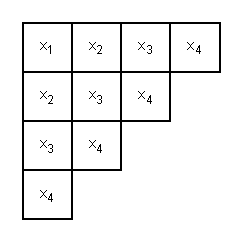
\includegraphics[width=0.25\textwidth]{bitwise-sorting-akers.pdf}
\caption[Akers array for binary sorting]{\centering Akers array for bit-wise sorting \cite{f1ed133a92fb4968b15110edea392daa}
\label{fig:Bit-wise-sorting}}
\end{figure}

% The golden model for this kind of binary-sorting Akers array can be simulated using high-level languages for testing purposes.

\section{Generalized sorting}{\label{sec:gen-sorting}}
\medskip
\subsection{Sorting with non-binary Akers Array}{\label{subsec:gsort-nb-akers-array}}
\medskip
Previous scientific research \cite{6620650} explores that the properties of binary Akers arrays can be theoretically extended to non-binary Akers arrays with some additional features. To sort \( n \) numbers, $\frac{n \times (n + 1)}{2}$ basic cells are required. Figure \ref{fig:Non binary Akers array} illustrates such a scenario with 4 non-binary symbols which requires $\frac{4 \times (4 + 1)}{2} = 10$ cells. The non-binary alphabets can be considered as $\mathcal{A} = \{0, 1, 2, \ldots, q-1\}$ where $q \in \mathbf{Z}^+$.

\medskip

The basic cell output can be defined as a function, $f(x, y, z): \mathcal{A}^3 \to \mathcal{A}$, given by:
\[
f = \text{median}(x, y, z)
\]

All cells of the leftmost column take $q-1$ as the $y$ (left) input. Conversely, all cells of the topmost row receive $0$ as the $x$ (top) input. The numbers to be sorted are provided as the variable inputs \( z \). It can be observed from Figure \ref{fig:Non binary Akers array} that $[z_0, z_1, z_2, z_3]$ is the sequence to be sorted and $[f_3, f_6, f_8, f_9]$ is the sorted sequence.
% \medskip 
% \[
% \frac{n \times (n + 1)}{2}
% \]

\medskip

\begin{figure}[h]
\centering
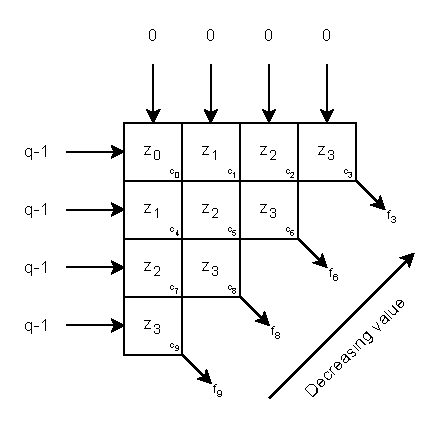
\includegraphics[width=0.4\textwidth]{nb-sort.pdf}
\caption[Non-binary Akers array]{\centering Non-binary Akers array
\label{fig:Non binary Akers array}}
\end{figure}

% The required number of cells:
% \[
% \frac{4 \times (4 + 1)}{2} = 10
% \]

% Each cell's output is determined by calculating the median of its three inputs:
% \[
% f = \text{med}(x, y, z)
% \]

The following two examples (in octal number system) illustrate the sorting. 

\textit{Example 1}: Let \( z_0 = 6 \), \( z_1 = 3 \), \( z_2 = 4 \), and \( z_3 = 1 \). The sorted output yields:
\[
f_3 = 1, \quad f_6 = 3, \quad f_8 = 4, \quad \text{and} \quad f_9 = 6
\]

The $f$ for individual cells are shown in Table \ref{table:example-1}.

\begin{table}[h]
\caption{\centering The $f$ for Example 1\label{table:example-1}}
\centering
\begin{tabular}{|c|c|}
\hline
\textbf{$\#cell$} & \textbf{$output$} \\
\hline $0$ & $6$ \\
\hline $1$ & $3$ \\
\hline $2$ & $3$ \\
\hline $3$ & $1$ \\
\hline $4$ & $6$ \\
\hline $5$ & $4$ \\
\hline $6$ & $3$ \\
\hline $7$ & $6$ \\
\hline $8$ & $4$ \\
\hline $9$ & $6$ \\
\hline
\end{tabular}
\end{table}

\textit{Example 2}: Let \( z_0 = 1 \), \( z_1 = 4 \), \( z_2 = 3 \), and \( z_3 = 6 \). The sorted output:
\[
f_3 = 1, \quad f_6 = 3, \quad f_8 = 4, \quad \text{and} \quad f_9 = 6
\]
The $f$ for individual cells are shown in Table \ref{table:example-2}.

\begin{table}[h]
\caption{\centering The $f$ for Example 2\label{table:example-2}}
\centering
\begin{tabular}{|c|c|}
\hline
\textbf{$\#cell$} & \textbf{$output$} \\
\hline $0$ & $1$ \\
\hline $1$ & $1$ \\
\hline $2$ & $1$ \\
\hline $3$ & $1$ \\
\hline $4$ & $4$ \\
\hline $5$ & $3$ \\
\hline $6$ & $3$ \\
\hline $7$ & $4$ \\
\hline $8$ & $4$ \\
\hline $9$ & $6$ \\
\hline
\end{tabular}
\end{table}

% In the leftmost column, the input \( Y \) is set to \( q - 1 \). For example, in the octal system, where \( q = 8 \), we have \( q - 1 = 7 \). The possible values of the variables are \( 0, 1, 2, 3, 4, 5, 6, 7 \).

% Let \( x_1, x_2, \ldots, x_n \) be \( n \) non-binary alphabets. A sorting array can be constructed with these values such that the outputs are given by:

% \[
% f_{1,n}, f_{2,n-1}, \ldots, f_{n,1}
% \]

% These outputs satisfy the following conditions:

% 1. 
% \[
% x_1, x_2, x_3, \ldots, x_n = f_{1,n}, f_{2,n-1}, \ldots, f_{n,1}
% \]
% 2. 
% \[
% f_{1,n} \leq f_{2,n-1} \leq \ldots \leq f_{n,1}
% \]

% To illustrate, consider four variables \( x_1, x_2, x_3, x_4 \) defined as \( x_1 = 2, x_2 = 4, x_3 = 5, x_4 = 6 \). We will use 10 cells to compute the outputs:

% \begin{align*}
% \text{Cell } c_1: & \quad f = \text{med}(2, 7, 1/0) = 2 \\
% \text{Cell } c_2: & \quad \text{inputs } (2, 7, 1/0) \implies f = 2 \\
% \text{Cell } c_3: & \quad \text{inputs } (2, 7, 1/0) \implies f = 2 \\
% \text{Cell } c_4: & \quad \text{inputs } (2, 7, 1/0) \implies f = 2 \\
% \end{align*}
% Thus, we have:

% \[
% f_1 = 2
% \]

% Continuing similarly for the next values, we find:

% \[
% f_2 = 4, \quad f_3 = 5, \quad f_4 = 6
% \] 

\subsection{Using binary Akers array}{\label{subsec:gsort-b-akers-array}}
\medskip
The generalized sorting described in Section \ref{subsec:gsort-nb-akers-array} demands the computation of $median(x, y, z)$. This section realizes generalized sorting with binary Akers array. Here, the elements of the input list are sorted in $n$-bit binary format.
\medskip

The 1\textsuperscript{st} step of sorting a list of numbers (elements) is a comparison between two numbers. Let assume two $n$-bit binary numbers:
\begin{itemize}
     \item $A = A_{n-1}A_{n-2} \ldots A_1A_0$
     \item $B = B_{n-1}B_{n-2} \ldots B_1B_0$
\end{itemize}

The numbers to be sorted are linearly stored in memory.

The $i^{th}$ bits of A and B - that is, $A_i$ and $B_i$ are compared. The truth table for $A_i > B_i$ is shown in Table \ref{table:Ai-gt-Bi}.

\begin{table}[h]
\caption{\centering Truth table for $A_i > B_i$\label{table:Ai-gt-Bi}}
\centering
\begin{tabular}{|c|c|c|}
\hline
\textbf{$A_i$} & \textbf{$B_i$} & \textbf{$A_i > B_i$} \\
\hline $0$ & $0$ & $0$ \\
\hline $0$ & $1$ & $0$ \\
\hline $1$ & $0$ & $1$ \\
\hline $1$ & $1$ & $0$ \\
\hline
\end{tabular}
\end{table}

% Karnaugh maps of this operation (in order to optimize) for both SOPs (sum of products) and POSs (product of sums) forms as per \textquotedblleft A synthesis procedure\textquotedblright\cite{5009040} is considered in Fig. \ref{fig:KarnaughMap-gt}, as follows:

The SOPs (sum of products) $A_iB_i$ and POSs (product of sums) of $A_i$ and $B_i$ are derived using Karnaugh maps as shown in Figure \ref{fig:KarnaughMap-gt}.

\begin{figure}[h]
\centering
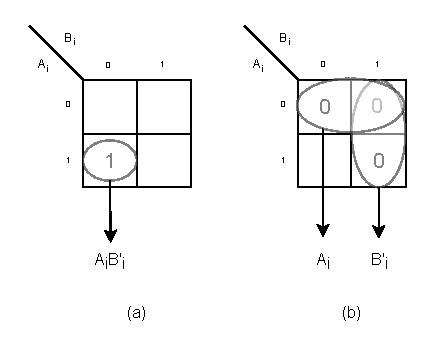
\includegraphics[width=0.40\textwidth]{kmap01.pdf}
\caption[K-maps for bitwise \textquotedblleft $>$\textquotedblright 
 $ $ comparison]{\centering K-maps for $A_i > B_i$ in (a) SOP and (b) POS forms
\label{fig:KarnaughMap-gt}}
\end{figure}

% It can be observed that the SOPs form results in only one term --- $A_iB'_i$.
% Alternatively, POSs form has two terms --- $A_i$, and $B'_i$.

% \bigskip

In Table \ref{tab:ai-bi} the SOPs ($1$s) are assigned as \textquotedblleft row headers\textquotedblright, and the POSs ($0$s) are assigned as the \textquotedblleft column headers\textquotedblright $ $ . The table entries are:

$\mathit{entry_{pq} = commonLiteral(rowHeader_p, columnHeader_q)}$

\medskip

\begin{table}[h]
    \caption{\centering Synthesis of $A_i > B_i$ \label{tab:ai-bi}}
    \centering
    \begin{tabular}{c|cc}
    % \toprule
    \textbf{ } & \bm{$A_i$} & \bm{$B'_i$} \\
    \hline
    \bm{$AB'_i$} & $A_i$ & $B'_i$ \\
    \hline
    \end{tabular}
\end{table}

This structure can be used as the premise for the \textquotedblleft synthesis\textquotedblright $ $ (introduced in \cite{5009040}) and shown in Figure \ref{fig:Akers1}.

% \bigskip

The fields (entries) only, part of Table \ref{tab:ai-bi} are considered as the Akers array combination for evaluating $A_i > B_i$. The $f_i$ in Figure \ref{fig:Akers1} represents the outcome of this comparison.

\begin{figure}[h]
\centering
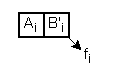
\includegraphics[width=.15\textwidth]{akers1.pdf}
\caption[Akers array for $A_i > B_i$]{\centering Akers array for $f_i = A_i > B_i$
\label{fig:Akers1}}
\end{figure}

% \bigskip

% The following enables the realization of $A_{n-1:0} > B_{n-1:0}$:
It can be observed that $\forall i \in \{n-1, n-2, \ldots, 1, 0\}$, $f_i$ can be computed in parallel. Now, there are two ways to proceed.

\medskip

In the $1^{st}$ approach, the most significant bit pairs of $A$ and $B$ is compared first. If the decision ($A > B$) is found, there is no need to compare the least significant bits. It removes the need for \textquotedblleft parallel comparison\textquotedblright $ $ of all corresponding bit pairs.

% The $1^{st}$ approach --- higher corresponding bit pairs of $A$ and $B$ can be compared earlier. If the decision result ($A > B$) is found, there is no need to go and compare the lower bits. It removes the need for \textquotedblleft parallel comparison\textquotedblright $ $ of all corresponding bit pairs.

\medskip
The $2^{nd}$ approach takes all the results of the parallel comparisons and uses a final linear Akers array, with space complexity $\mathcal{O}(n)$, to get the final result. This $n$ stands for the $n$-bit numbers.

\medskip

The branch divergence problem can be found in the $1^{st}$ approach, and that can be solved using the $2^{nd}$ approach \cite{10.1145/1964179.1964184}. Taking all these into consideration, the $2^{nd}$ approach is provided for the current work. The 1-bit final comparison result $g = A_{n-1:0} > B_{n-1:0}$ can be computed as illustrated in Figure \ref{fig:Akers2}.

\medskip

\textit{Theorem 1:} The Akers array illustrated in Figure \ref{fig:Akers2} implements the function
$\alpha(z_0,\ldots,z_{n-1})$ $ :\{0,1\}^n \to \{0, 1\}$, as given by:
\begin{align}
    \alpha = z_{n-1} \vee (z_{n-1}'\wedge z_{n-2}) \vee (z_{n-1}' \wedge z_{n-2}' \wedge z_{n-3}) \vee \nonumber
    \\
    \ldots \vee ((\bigwedge_{i=1}^{n-1} z_i') z_0) \label{eq:col-array}
\end{align}

\textit{Proof 1:} According to S. B. Akers \cite{5009040}, the $z$-input of $0$ to a single Akers array cell results in row elimination, whereas $1$ as the $z$-input results in column elimination and the outputs of each cell of such a row and each cell of such a column are 0 and 1, respectively. For the array in Figure \ref{fig:Akers2}, $z$ inputs are given by $z_i = f_i$. In the topmost cell, the $z$ input is $f_{n-1}$. If $f_{n-1} = 1$, using column elimination, the output $g = 1$. Otherwise, if $f_{n-1} = 0$, row elimination is performed, and so, rest of the array should be considered. This gives the $1^{st}$ component of the sum in equation \ref{eq:col-array}. The $2^{nd}$ cell from the top would be considered only if $f_{n-1} = 0$. Therefore, it gives the $2^{nd}$ component $f_{n-1}'f_{n-2}$. Likewise, moving downwards in the same manner, we can obtain the rest of the components.

\medskip

\begin{figure}[h]
\centering
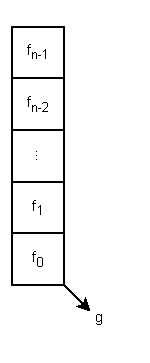
\includegraphics[width=0.13\textwidth]{akers2.pdf}
\caption[Akers array for $A > B$]{\centering Akers array for $g = A_{n-1:0} > B_{n-1:0}$
\label{fig:Akers2}}
\end{figure}

% So, we found the result $g = (A > B)$ ($1$-bit).

% \bigskip

% --- What were we supposed to do with it?

The $g$ is utilized in an analogous style as the \textquotedblleft select\textquotedblright $ $ for the \textquotedblleft mux\textquotedblright $ $ (multiplexing) operations ($n$-bit 2-1 mux) to determine the greater and the smaller one between $A$ and $B$:
    \begin{align}
        Y_{n-1:0} = \mathit{max(A_{n-1:0}, B_{n-1:0})}
    \end{align}\label{eq:full-max}
    \begin{align}
        X_{n-1:0} = \mathit{min(A_{n-1:0}, B_{n-1:0})}
    \end{align}\label{eq:full-min}

For a single bit, say $i^{th}$, 
    \begin{align}
        Y_i = max(A_i, B_i) = g'B_i + gA_i \label{eq:indiv-max}
    \end{align}

Similarly, 
    \begin{align}
        X_i = min(A_i, B_i) = gB_i + g'A_i \label{eq:indiv-min}
    \end{align}

Table \ref{tab:3} represents the truth table for Equation \ref{eq:indiv-min}.
\begin{table}[h]
    \caption{\centering Truth table for $Y_i = g'B_i + gA_i$}
    \centering
    \begin{tabular}{|ccc|c|}
        \hline
        \textbf{$g$} & \textbf{$A_i$} & \textbf{$B_i$} & \textbf{$Y_i$} \\
        \hline 
        $0$ & $0$ & $0$ & $0$ \\
        $0$ & $0$ & $1$ & $1$ \\
        $0$ & $1$ & $0$ & $0$ \\
        $0$ & $1$ & $1$ & $1$ \\
        $1$ & $0$ & $0$ & $0$ \\
        $1$ & $0$ & $1$ & $0$ \\
        $1$ & $1$ & $0$ & $1$ \\
        $1$ & $1$ & $1$ & $1$ \\
        \hline
    \end{tabular}
    \label{tab:3}
\end{table}

The K-maps for the expression $Y_i = g'B_i + gA_i$ in its SOPs and POSs forms are shown in Figure \ref{fig:Kmap-y-SOPs} and \ref{fig:Kmap-y-POSs}, respectively. The \textquotedblleft synthesis\textquotedblright $ $ of $Y_i = g'B_i + gA_i$ is shown in Table \ref{tab:synth2}.

\begin{figure}[h]
    \centering
    \begin{subfigure}[b]{0.4\textwidth}
        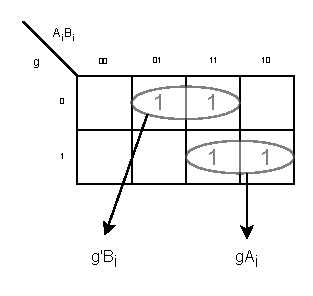
\includegraphics[width=0.85\linewidth]{kmap02-SOPs.pdf}
        \caption[$SOPs$]{$SOPs$
        \label{fig:Kmap-y-SOPs}}
    \end{subfigure}
    % \centering
    \begin{subfigure}[b]{0.4\textwidth}
        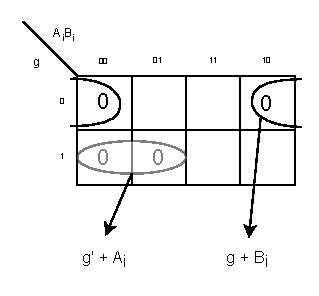
\includegraphics[width=0.85\linewidth]{kmap02-POSs.pdf}
        \caption[$POSs$]{$POSs$
        \label{fig:Kmap-y-POSs}}
    \end{subfigure}
    \caption[K-maps for $g'B_i + gA_i$]{\centering K-maps for $g'B_i + gA_i$ in (a) SOPs and (b) POSs\label{fig:Kmap-y}}
\end{figure}

\begin{table}[h]
    \caption{\centering Synthesis of $Y_i = g'B_i + gA_i$}
    \centering
    \begin{tabular}{c|cc}
    % \toprule
    \textbf{ } & \bm{$g + B_i$} & \bm{$g' + A_i$} \\
    \hline
    \bm{$g'B_i$} & $B_i$ & $g'$ \\
    % \hline
    \bm{$gA_i$} & $g$ & $A_i$ \\
    % \bottomrule 
    \hline
    \end{tabular}
    \label{tab:synth2}
\end{table}

It enables us to create the Akers array for $Y_i = max(A_i, B_i)$ as depicted in Figure \ref{fig:Akers3a}. Similarly, we can obtain the Akers' array for $X_i = min(A_i, B_i)$ as shown in Figure \ref{fig:Akers3b} can be obtained.
\begin{figure}[h]
    \centering
    \begin{subfigure}[b]{0.2\textwidth}
        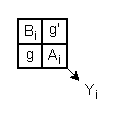
\includegraphics[width=0.7\linewidth]{akers3.pdf}
        \caption[$max(A_i, B_i)$]{$Y_i = max(A_i, B_i)$
        \label{fig:Akers3a}}
    \end{subfigure}
    % \centering
    \begin{subfigure}[b]{0.2\textwidth}
        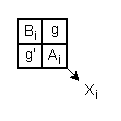
\includegraphics[width=0.7\linewidth]{akers4.pdf}
        \caption[$min(A_i, B_i)$]{$X_i = min(A_i, B_i)$
        \label{fig:Akers3b}}
    \end{subfigure}
    \caption[Akers' array for $min$ and $max$]{\centering Akers' array for $min$ and $max$}
    {\label{fig:Akers3}}
\end{figure}

There can be the parallel (spatial) realization of the max/min operations for all the $n$-bit pairs. Now, the task is to overwrite $A$ with $X$, and $B$ with $Y$.

\bigskip
% \newpage

Now, various general-purpose sorting algorithms can be realized with the Akers array. implemented. For simplicity, the bubble sort is considered for the current work.

\begin{figure}[h]
\centering
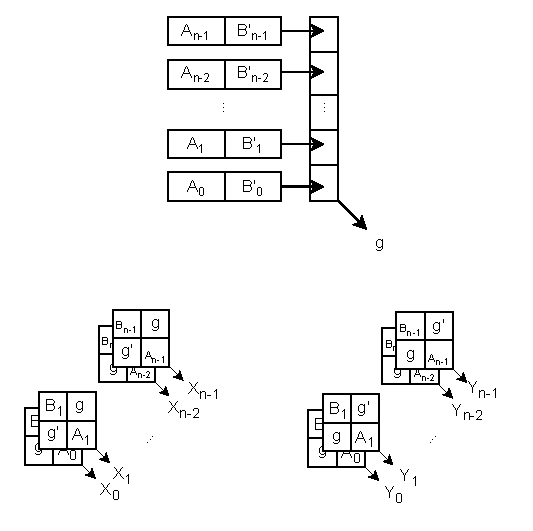
\includegraphics[width=0.45\textwidth]{final.pdf}
\caption[Overall operation]{\centering Overall operations [$X = min(A, B)$, $Y = max(A, B)$]
\label{fig:final}}
\end{figure}

Suppose, four linearly organized $4$-bit numbers ---
\begin{enumerate}
    \item $P = P_3P_2P_1P_0$
    \item $Q = Q_3Q_2Q_1Q_0$
    \item $R = R_3R_2R_1R_0$
    \item $S = S_3S_2S_1S_0$
\end{enumerate}

Let consider that the unsorted list is $[P, Q, R, S]$.

\medskip

\textit{First pass}: the entire process (the procedure illustrated in Figure \ref{fig:final} and the overwrite operation) is performed on $P$ and $Q$. Let this results in $P'$ in place of $P$ and $Q'$ in place of $Q$. After that, it is applied on $Q'$ and $R$ which produces $Q^{''}$ and $R'$ replacing $Q'$ and $R$, respectively, if applicable. Finally, it is applied on $R'$ and $S$, yields $R^{''}$ and $S'$ in the given order.

Therefore, after the first pass, the sequence becomes $[P', Q^{''}, R^{''}, S']$. According to the bubble sort algorithm, the fourth number, i.e. $S'$, is in the correct position. That is why there is no need to consider the fourth number in the next pass.

\medskip

\textit{Second pass}: The entire process, as in first pass, is applied on $P'$ and $Q^{''}$ yielding $P^{''}$ and $Q^{'''}$. Next, $Q^{'''}$ and $R{''}$ undergo the same process and leads to $Q^{''''}$ and $R^{'''}$.

Consequently, after the second pass, the resulting sequence is $[P^{''}, Q^{''''}, R^{'''}, S']$. This time, the third number, i.e., $R^{'''}$ is in the correct position so, it is skipped in the next pass.

\medskip

\textit{Third pass}: once again the process is carried out on $P^{''}$ and $Q^{''''}$ yielding $P^{'''}$ and $Q^{'''''}$ respectively.Eventually, the sequence after third pass becomes $[P^{'''}, Q^{'''''}, R^{'''}, S']$. In this instance, the second number, i.e., $Q^{'''''}$, is in the correct position. Therefore, it can be skipped. Additionally, according to the bubble sort algorithm, a single element is always sorted. So, no extra passes will be needed for the remaining number.

\medskip

The sorting concludes and the sorted sequence is $[P^{'''}, Q^{'''''}, R^{'''}, S']$.

\medskip

% \newpage

\section{In-Memory Searching in Akers array}{\label{sec:search}}

% \subsection{Using binary Akers array}

Here, two $n$-bit numbers, $A$ and $B$, are considered in a manner similar to that in Section \ref{subsec:gsort-b-akers-array}. Let us further assume that $A$ is one of the \textquotedblleft keys\textquotedblright $ $ and $B$ is the \textquotedblleft query\textquotedblright $ $ of this \textquotedblleft search\textquotedblright $ $ procedure. The $i^{th}$ bits of A and B, i.e., $A_i$ and $B_i$, are compared to check whether they are equal. The truth table for $A_i = B_i$ is represented as Table \ref{table:Ai-eq-Bi}.

\begin{table}[h]
\caption{\centering Truth table for $A_i = B_i$\label{table:Ai-eq-Bi}}
\centering
\begin{tabular}{|c|c|c|}
\hline
\textbf{$A_i$} & \textbf{$B_i$} & \textbf{$A_i = B_i$} \\
\hline $0$ & $0$ & $1$ \\
\hline $0$ & $1$ & $0$ \\
\hline $1$ & $0$ & $0$ \\
\hline $1$ & $1$ & $1$ \\
\hline
\end{tabular}
\end{table}

\begin{table}[h]
    \caption{\centering Synthesis of $A_i = B_i$}
    \centering
    \begin{tabular}{c|cc}
    % \toprule
    \textbf{ }   & \bm{$A_i'+B_i$} & \bm{$A_i+B_i'$} \\
    \hline
    \bm{$A_i'B_i'$} & $A_i'$ & $B_i'$ \\
    % \hline
    \bm{$A_iB_i$}  & $B_i$ & $A_i$ \\
    % \bottomrule 
    \hline
    \end{tabular}
    \label{tab:synth-ai-eq-bi}
\end{table}

As in Section \ref{subsec:gsort-b-akers-array}, are carried out here. In this case, the obtained SOPs are --- i) $A_i'B_i'$, and ii) $A_iB_i$. On the other hand, the POSs are --- i) $A_i'+B_i$, and ii) $A_i+B_i'$. The synthesized Akers array for $A_i=B_i$, following Table VIII is illustrated in Figure \ref{fig:akers-ai-eq-bi}.

\begin{figure}[h]
\centering
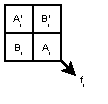
\includegraphics[width=0.18\textwidth]{akers-equality-bitwise.pdf}
\caption[Akers array for $A_i = B_i$]{\centering Akers array for $A_i = B_i$
\label{fig:akers-ai-eq-bi}}
\end{figure}

The process enables to design Akers logic circuit for all $n$ pair of bits of $A$ and $B$. The bit pairs are compared in parallel. These $n$ comparison results are then chained together in Akers array as depicted in Figure \ref{fig:akers-a-eq-b} to obtain the final result $g$.

\medskip

\textit{Theorem 2:} The Akers array illustrated in Figure \ref{fig:akers-a-eq-b} implements the function
$\beta(z_0,\ldots,z_{n-1})$ $ :\{0,1\}^n \to \{0, 1\}$, as given by:

\begin{align}
    \beta = z_0 \wedge (z_0'\vee z_1) \wedge (z_0' \vee z_1' \vee z_2) \wedge \nonumber
    \\
    \ldots \wedge ((\bigvee_{i=0}^{n-2} z_i') z_{n-1}) \nonumber \\
    = z_0 \wedge z_1 \wedge z_2\wedge \ldots \wedge z_{n-2} \wedge z_{n-1}
    \label{eq:row-array}
\end{align}

The proof of this equation can be produced in a way very similar to that of the Equation \ref{eq:col-array}.

\begin{figure}[h]
\centering 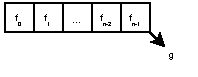
\includegraphics[width=0.32\textwidth]{akers-equality-chain.pdf}
\caption[Akers array for $g = (A_{n-1:0} = B_{n-1:0})$]{\centering Akers array for $g = (A_{n-1:0} = B_{n-1:0})$
\label{fig:akers-a-eq-b}}
\end{figure}

The overall process is illustrated in Figure \ref{fig:akers-a-eq-b-overall}. It could be considered as a \textquotedblleft partial\textquotedblright $ $ search because the query is supposed to be matched with all the keys that are present.

\begin{figure}[h]
\centering 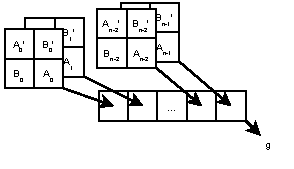
\includegraphics[width=0.38\textwidth]{akers-equality.pdf}
\caption[Overall comparison operation]{\centering Overall comparison operation for searching
\label{fig:akers-a-eq-b-overall}}
\end{figure}

Applying this process to each of the keys would vary from case to case. It could be done in a linear manner or even in parallel. 

The \textquotedblleft complete search\textquotedblright $ $ consists of \textquotedblleft partial search\textquotedblright $ $ of the \textquotedblleft query\textquotedblright $ $ with each of the keys, followed by a final Akers array operation --- to combine the results obtained by all the \textquotedblleft partial searches\textquotedblright $ $ and to decide if any of them is succeeded. This final step is depicted in Figure \ref{fig:akers-search}. The figure assumes the presence of $m$ keys, say, \{$K_0$, $K_1$, \ldots, $K_{m-2}$, $K_{m-1}$\}. The \textquotedblleft partial search\textquotedblright $ $ with \textquotedblleft key\textquotedblright $ $ $K_i$ gives the output $g_i$. In this case, $g_i$ is the $z$ input of the $i^{th}$ cell ($0$-indexed) of the Akers array depicted in Figure \ref{fig:akers-search}. The final result of the \textquotedblleft complete search\textquotedblright $ $ operation is $h$. 

\begin{figure}[h]
\centering 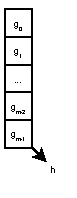
\includegraphics[width=0.11\textwidth]{akers-search-final.pdf}
\caption[The complete search operation]{\centering The complete search operation
\label{fig:akers-search}}
\end{figure}

% \subsection{Using memristive Akers array}

% Memristive Akers array, as a model for memory, supports \textquotedblleft read\textquotedblright $ $ and \textquotedblleft write\textquotedblright $ $ operations \cite{f1ed133a92fb4968b15110edea392daa}. Using the memristive Akers array as the base, we try to experiment with \textquotedblleft search\textquotedblright $ $ operations on it. We follow two such approaches. In the first case, we perform linear search. In the second case, we go for binary search after we perform the sorting as explained in section IV-B. For simplicity, let us consider the following sorted array depicted in Fig. \ref{fig:sorted-array}.

% \begin{figure}[h]
% \centering
% 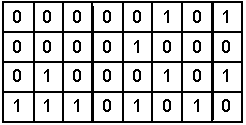
\includegraphics[width=0.2\textwidth]{sorted_array.pdf}
% \caption[Sorted memristive Akers array]{\centering $4\times8$ sorted memristive Akers array
% \label{fig:sorted-array}}
% \end{figure}

% Let us assume that the array stores four 8-bit unsigned integers in the range $[0-255]$:
% \begin{align*}
% 8'b0000\_0101 &= 3'd5, \\
% 8'b0000\_1000 &= 3'd8, \\
% 8'b0100\_0101 &= 3'd69, \\
% 8'b1110\_1010 &= 3'd234
% \end{align*}

% Also, say, the target is to search for $x$ (key, the unsigned integer). The \textquotedblleft search\textquotedblright $ $ is a composite operation that requires two relatively fundamental operations as a basis. The first is to \textquotedblleft read\textquotedblright $ $ an entire number from the array. It can be achieved using the row and column decoder of a 2M4T (2 memristors, 4 transistors) Akers array\cite{f1ed133a92fb4968b15110edea392daa}. The second is to \textquotedblleft compare\textquotedblright $ $ the number obtained by \textquotedblleft read\textquotedblright $ $ with the key. An Akers array similar to Fig. \ref{fig:Akers2} can be created to perform the \textquotedblleft compare\textquotedblright $ $ operation.

% \subsubsection{Linear Search}
% In this approach, the \textquotedblleft search\textquotedblright $ $ operation is iterated linearly, i.e., reading and comparing the numbers in the array one by one. The index (\textit{row}) selection can be done using the row decoder. Taking the all 8-bits of an entire number in the array for \textquotedblleft read\textquotedblright $ $ is performed using the column decoder\cite{f1ed133a92fb4968b15110edea392daa}. The \textquotedblleft search\textquotedblright $ $ starts at index-0. At the end of each unsuccessful \textquotedblleft read\textquotedblright $ $ and \textquotedblleft compare\textquotedblright $ $ combination, the number in the next index is visited until index-3 is reached.

% \subsubsection{Binary Search}
% Binary search is only sensible on a sorted array. The procedure may be better explained using a direct example. Let us assume that the target $x$ of the \textquotedblleft search\textquotedblright $ $ operation is $3'd7$. In this case, two indices are considered at the beginning of the procedure, the start index and the end index. Initially, the start index is 0, and the end index is 3.

% During the first iteration, the middle index is computed as $\lfloor\frac{\text{start-index } + \text{ end-index}}{2}\rfloor$ $= \lfloor\frac{0+3}{2}\rfloor$ $= \lfloor1.5\rfloor$ $= 1$. The value at the middle index, i.e., index-1, is $3'd8$. It is greater than the target value $3'd7$. So, the end index is updated to $(\text{middle-index} - 1)$ $= (1 - 1) = 0$.

% In the next iteration, the middle index is $\lfloor\frac{0+0}{2}\rfloor$ $= 0$. The value at the middle index ($0$) is $3'd5$. It is smaller than the target. So, the start index is updated to $(\text{middle-index + 1})$ $= (0 + 1)$ $= 1$. At this point, as the start index ($1$) is greater than the end index ($0$), the procedure is terminated.

% The result of the procedure is that the \textquotedblleft search\textquotedblright $ $ was unsuccessful because there was no match.

\medskip

\section{realization of in-memory computation}

This section reposts the realization of the Akers array based sorting/searching in-memory. This realization propose partitioning of the Akers array memory structure into two sections. Each of these sections has some operations to perform.

The first section supports read/write of data. No further operation would be allowed in this partition. For reference, let us call this section \textbf{Stasis}.

The second section inherits all the properties of the first section and also realizes the elementary cell operations of Akers array. Let us call this section \textbf{Flux}.

In a normal situation, the combined Stasis and Flux sections could behave as memory array. But, if required, the additional properties of the Flux section are triggered.

A simplistic illustration for such a partition is given by Figure \ref{fig:partition-array}. This part opens up new avenues of experimentation.

\begin{figure}[h]
\centering
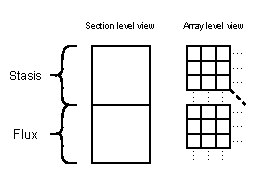
\includegraphics[width=0.4\textwidth]{section-akers.pdf}
\caption[Partition of memory array]{\centering Partition of memory array
\label{fig:partition-array}}
\end{figure}

The Flux section is further partitioned into a few subsections based on the particular shapes of the required Akers arrays.

Along the way through the sections \ref{sec:gen-sorting} and \ref{sec:search}, we utilized Akers arrays of the following shapes:
\begin{enumerate}
    \item{\label{shape:1}} $1 \times 2$
    \item $2 \times 2$
    \item $n \times 1$
    \item $1 \times n$
\end{enumerate}
Here, $n$ is the number of bits to represent an $n$-bit number. Furthermore, let us assume that the memory array is $n$-bit addressable. To make it simple and easy, $n$ could be $8$, turning it into a byte-addressable memory.

% subsection for 2x1

Such a subsection for $1 \times 2$ arrays is shown in Figure \ref{fig:1x2-array}. Each triggered $1 \times 2$ Akers array in this subsection would be padded with a column on the right and a row at the bottom - forming a $2 \times 3$ array block. The bottom-right cell would be chosen as the target cell from where the output of the array operation would be \textquotedblleft read\textquotedblright. This kind of setup is to avoid any inter-array data corruption.

\begin{figure}[h]
\centering
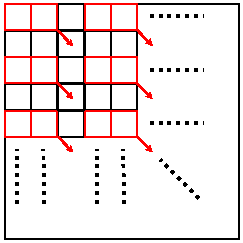
\includegraphics[width=0.2\textwidth]{subsection_2cross1.pdf}
\caption[The $1 \times 2$ array]{\centering The $1 \times 2$ array subsection
\label{fig:1x2-array}}
\end{figure}

% subsection for 2x2

Similarly, a subsection of $2 \times 2$ arrays is formed in Figure \ref{fig:2x2-array}. In this case, the blocks are $3 \times 3$ arrays. 

\begin{figure}[h]
\centering
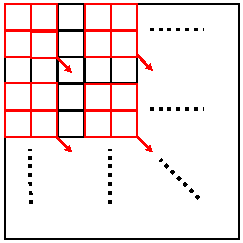
\includegraphics[width=0.2\textwidth]{subsection_2cross2.pdf}
\caption[The $2 \times 2$ array]{\centering The $2 \times 2$ array subsection
\label{fig:2x2-array}}
\end{figure}

% subsection for nx1
% subsection for 1xn

Figure \ref{fig:1xn-array} depicts a subsection for $1 \times n$ arrays. It requires a $2 \times n$ array to form a block. The $n \times 1$ array subsection is not required unless it would become strictly necessary because the $n \times 1$ array can be obtained by flipping all the external $x$ and $y$ inputs of the $1\times n$ array cells.

\begin{figure}[h]
\centering
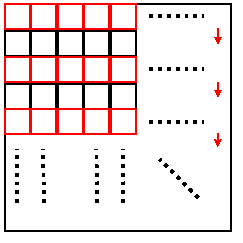
\includegraphics[width=0.2\textwidth]{subsection_1cross_n.pdf}
\caption[The $1 \times n$ array]{\centering The $1 \times n$ array subsection
\label{fig:1xn-array}}
\end{figure}

\medskip

\section{Conclusion}
% \medskip
This paper demonstrates how the Akers logic array can be effectively utilized for in-memory sorting and searching, leveraging its inherent parallelism and reconfigurable structure. By extending its capabilities to support both binary and non-binary data formats, the Akers array proves to be a flexible and powerful component for data-intensive operations. The comparative analysis of sorting mechanisms and the implementation of search strategies—both linear and binary—highlight the potential of Akers-based architectures in reducing memory bottlenecks and improving overall computational efficiency. Furthermore, the proposed in-memory model, featuring the Stasis and Flux partitioning, offers a conceptual pathway toward more dynamic and adaptable memory systems. These findings not only validate the utility of Akers arrays in current computing environments but also open up possibilities for future exploration in hardware-level optimizations for emerging data-centric applications.

\bibliography{references}
\bibliographystyle{ieeetr}


\begin{figure*}[!t]
    \centering
    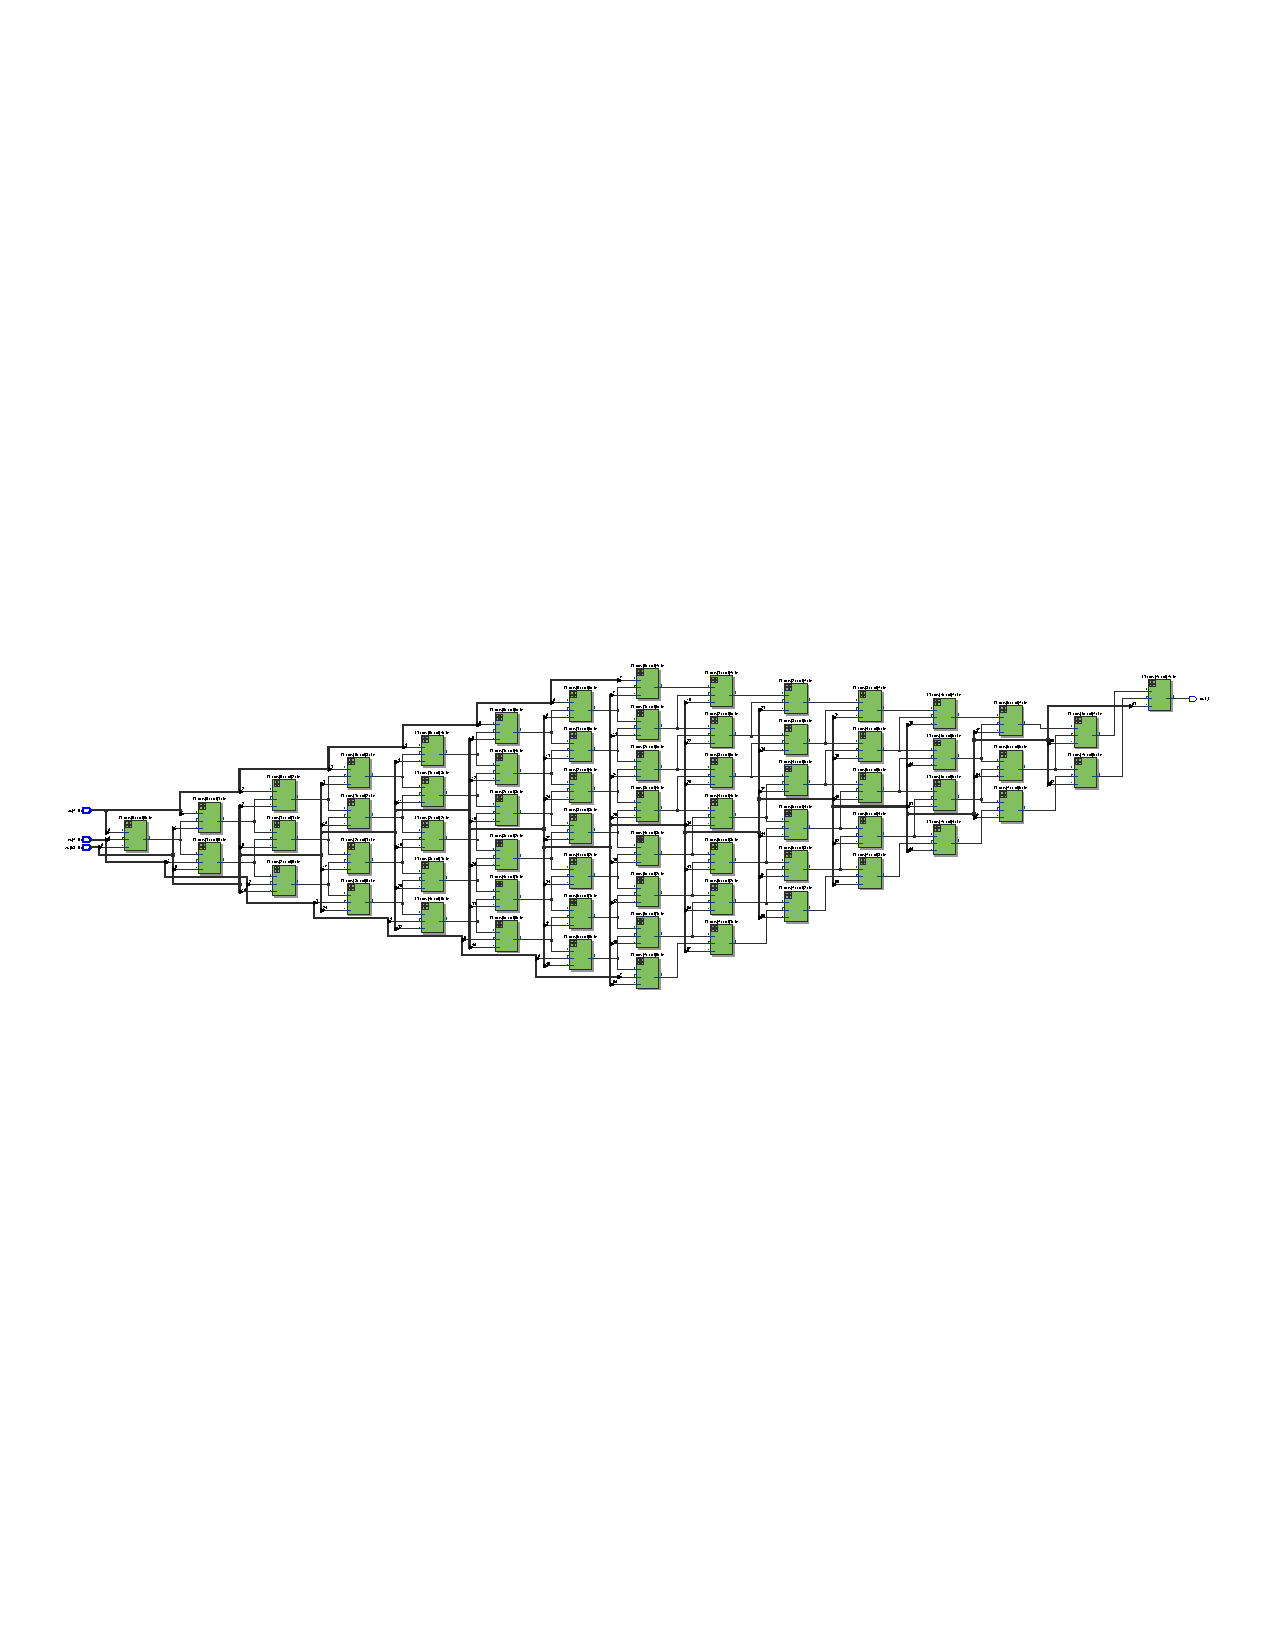
\includegraphics[scale=2, height=0.27\textheight, angle=-90]{akers_rtl_.pdf}
    \caption{$8\times8$ Akers array RTL design}
    \label{fig:large_diagram}
\end{figure*}


\end{document}
